
\section{Experiments}

This section first details our experiment setup, followed by a comparative analysis with state-of-the-art approaches. Subsequently, we present an ablation study to evaluate the efficacy of individual components in our proposed methods. Finally, we assess the computational efficiency of our approach, examine error cases, and evaluate the rendering quality.


\begin{table}[tb]
  \centering
  % Increase the padding of the columns
  % \setlength{\tabcolsep}{16pt}
  % Optionally, use a smaller font for the table
  \small
  \begin{tabular}{@{}l c c@{}}
    \toprule
    Method & Success~$\uparrow$ & SPL~$\uparrow$ \\
    \midrule
    RL Baseline \cite{krantz2022instancespecific} & 0.083 & 0.035  \\
    OVRL-v2 ImageNav \cite{yadav2023ovrl} & 0.006 & 0.002 \\
    OVRL-v2 IIN \cite{yadav2023ovrl} & 0.248 & 0.118 \\
    FGPrompt \cite{sun2024fgprompt} & 0.099 & 0.028 \\
    \midrule
    MultiON Baseline \cite{wani2020multion} & 0.066 & 0.045 \\
    MultiON Implicit \cite{marza2023multi} & 0.143 & 0.107 \\
    MultiON Camera \cite{chen2022learning} & 0.186 & 0.142 \\
    \midrule
    Mod-IIN \cite{krantz2023navigating} & 0.561 & 0.233 \\
    IEVE Mask RCNN \cite{lei2024instanceaware} & 0.684 & 0.241 \\
    IEVE InternImage \cite{lei2024instanceaware} & 0.702 & 0.252 \\
    \midrule
    Mod-IIN \cite{krantz2023navigating} (Scene Map) & 0.563 & 0.323 \\
    IEVE Mask RCNN \cite{lei2024instanceaware} (Scene Map) & 0.683 & 0.331 \\
    IEVE InternImage \cite{lei2024instanceaware} (Scene Map) & 0.705 & 0.347 \\
    \textbf{GaussNav (ours)} & \textbf{0.725} & \textbf{0.578}\\
    \bottomrule
  \end{tabular}
  % \vspace{-10pt}
  \vspace{5pt}
  \caption{Performance comparison of our GaussNav with previous state-of-the-art methods on the HM3D \cite{yadav2023habitat} datasets across two different metrics: Success and SPL \cite{anderson2018evaluation}. The table is divided into four sections. The first section presents the results of end-to-end methods. The second section shows the transfer performance of MultiON-related methods on the IIN task. The third section includes the state-of-the-art methods on the IIN task. Finally, the fourth section aims to provide a fair comparison with GaussNav by replacing the episodic map used in these methods from the third section with a scene-specific map, allowing the agent to retain the map from the previous episode.}
  \vspace{-18pt}
  \label{tab:main}
\end{table}

\subsection{Experiment Setup}

\textbf{Datasets.} We use Habitat-Matterport 3D dataset (HM3D) \cite{yadav2023habitat} in the Habitat \cite{szot2022habitat} for our experiments. HM3D consists of scenes which are 3D reconstructions of real-world environments with semantic annotations. These scenes are split into three distinct subsets for training, validation, and testing, consisting of 145/36/35 scenes, respectively. We follow the task setting of Instance ImageGoal Navigation (IIN) proposed by Krantz \etal \cite{krantz2022instancespecific}. The episode dataset has been partitioned into three subsets for training, validation, testing, comprising 7,056K/1K/1K episodes respectively. The object depicted by the goal image belongs to the following six categories:  \{``chair'', ``couch'', ``plant'', ``bed'', ``toilet'', ``television''\}. On the validation subset, a total of 795 unique object instances have been observed.

\textbf{Embodiment.} We adopt the embodiment parameters from the Hello Robot Stretch platform \footnote{\url{https://hello-robot.com/stretch-2}}. The simulated agent is modeled as a rigid-body cylinder with zero turning radius, a height of 1.41m, and a radius of 0.17m. A forward-facing RGB-D camera is affixed at a height of 1.31 m. At each timestep $t$, the agent's observation consists of an egocentric RGB image, depth image, goal image and sensor pose reading. Camera specifications, such as mounting height, look-at angle, and field of view (FOV), differ between the agent's and the goal's cameras. Specifically, the agent's camera resolution is $640\times480$, whereas the goal's camera has a resolution of $512\times512$ with unfixed height and FOV parameters.

\begin{figure}[tb]
\centering
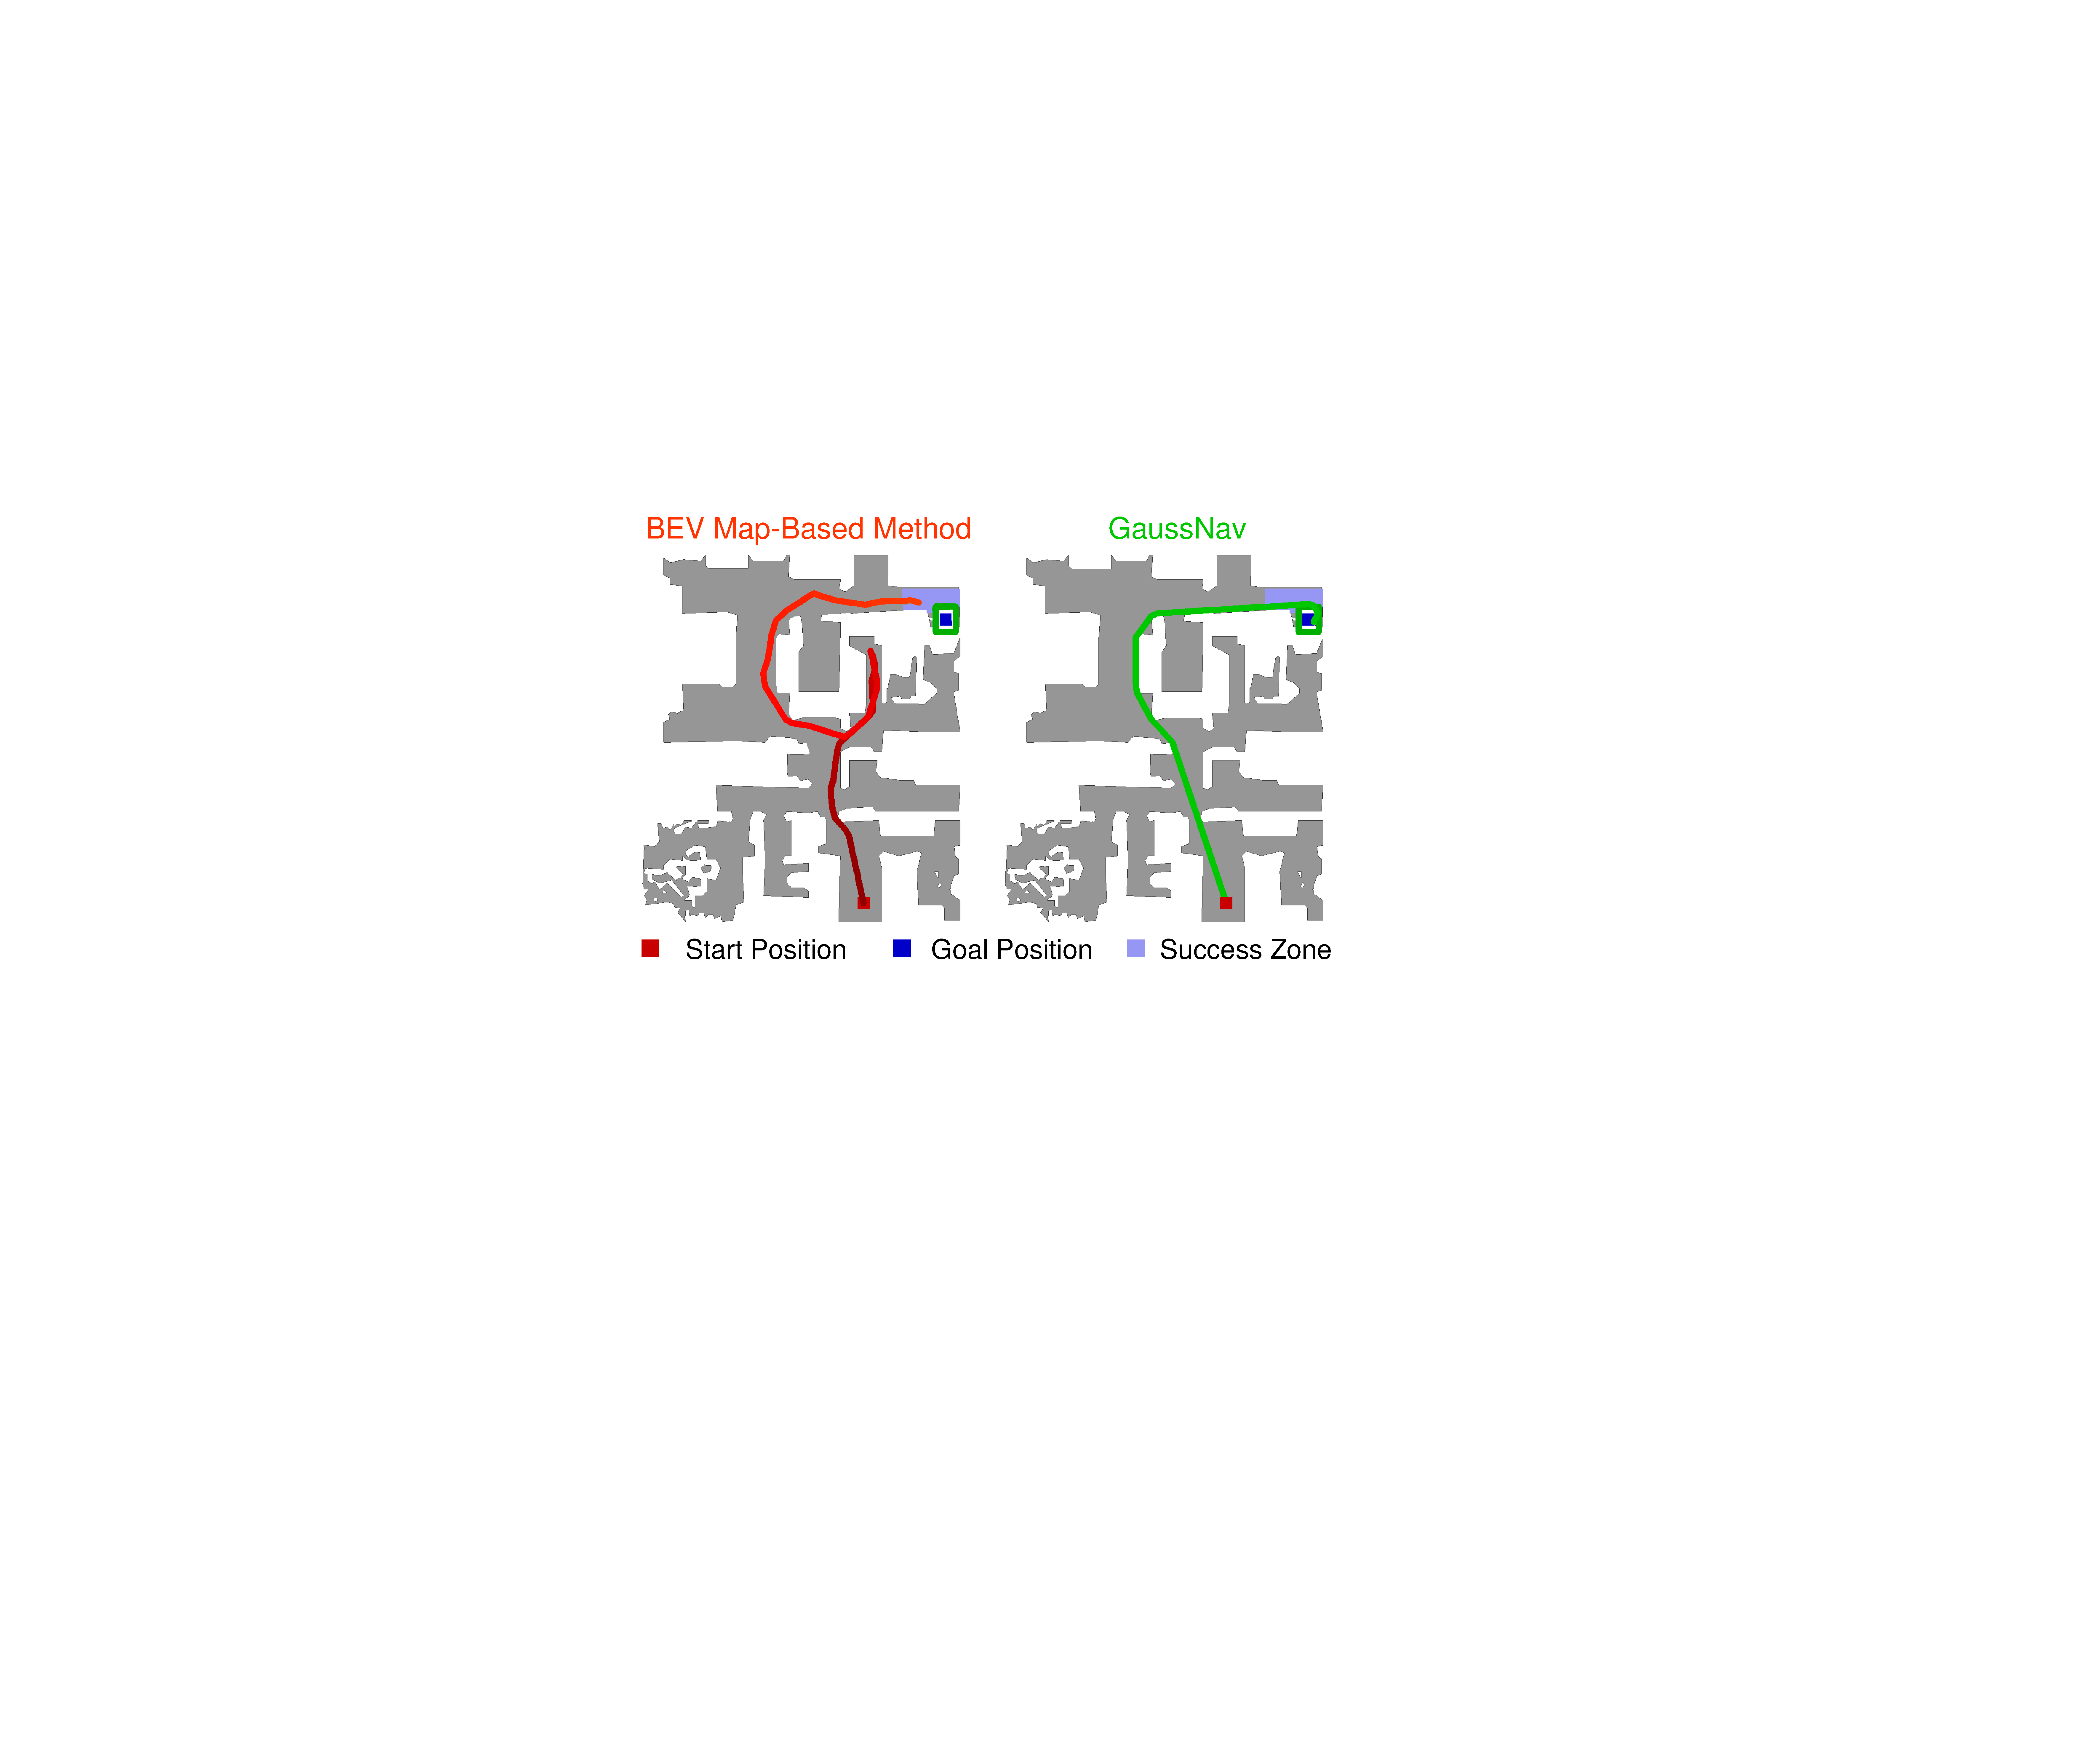
\includegraphics[width=0.45\textwidth]{pics/trajectory.pdf}
\caption{Trajectory Analysis. Our Semantic Gaussian map representation can allow agent to directly ground target object from a single goal image, thereby facilitating efficient visual navigation.}
\label{fig:trajectory}
\vspace{-10pt}
\end{figure}

\textbf{Action Space.} We use a discrete action space for navigation, comprising four actions: \{\texttt{STOP}, \texttt{FORWARD}, \texttt{TURN\_RIGHT}, \texttt{TURN\_LEFT}\}. The \texttt{STOP} action terminates the current episode, while the \texttt{FORWARD} action advances the agent by 25 cm. Rotational actions occur in place: \texttt{TURN\_RIGHT} induces a 25-degree clockwise rotation and \texttt{TURN\_LEFT} a 25-degree counter-clockwise rotation.

\textbf{Evaluation Metrics.} Following Krantz \etal \cite{krantz2022instancespecific}, we evaluate our model with both success and efficiency. We report Success Rate (Success), Success rate weighted by normalized inverse Path Length (SPL). An episode is deemed successful ($\text{Success} = 1$) if the agent invokes the \texttt{STOP} action within a $1.0$m Euclidean distance from the goal object. SPL is an efficiency measure defined in \cite{anderson2018evaluation}, is given by:
\begin{equation}
    \text{SPL} = \frac{1}{N} \sum_{i=1}^{N} S_i \cdot \frac{l_i}{\max(p_i, l_i)},
\end{equation}
where $N$ is the total number of episodes, $S_i$ is a binary success indicator for episode $i$, $l_i$ is the shortest path distance from the start position to the goal, and $p_i$ is the path length actually traversed by the agent. A higher SPL value indicates more efficient navigation.



\subsection{Comparison to the State-of-the-art Methods}

We evaluate our proposed model against various baselines and previous state-of-the-art work, as presented in \Cref{tab:main}. Unlike conventional IIN methods that generate a map for each episode, GaussNav constructs a map across episodes in a scene. The first block lists results from end-to-end baselines, and the second block includes methods designed for the MultiON task but implemented here for the IIN task. The third block of \Cref{tab:main} presents the performance of original state-of-the-art IIN methods, while the fourth block reports their performance when adapted to use scene map.

\textbf{End-to-end Baselines.} We evaluate the performance of two end-to-end methods on the IIN task. \textit{RL Baseline} built a network that observes agent RGB $(\mathcal{V}_{RGB})$, agent depth $(\mathcal{V}_{D})$, the goal image $(\mathcal{V}_G)$, GPS coordinates $(x,z)$, and heading $(\theta)$. Visual observations are encoded with separate ResNet-18~\cite{he2016deep} encoders and GPS and heading are encoded with 32-dimensional linear layers. Then, these features are concatenated and encoded with a 2-layer LSTM. Finally, an action $a(t)$ is sampled from a categorical distribution. The network was trained from scratch using Proximal Policy Optimization (PPO) \cite{schulman2017proximal}.

\textit{OVRL-v2}, proposed by Yadav \etal \cite{yadav2023ovrl}, introduced self-supervised pretraining for visual encoders in ImageGoal Navigation. Originally, OVRL-v2 was trained for the ImageGoal Navigation task. Direct application of OVRL-v2 to IIN task without fine-tuning yields suboptimal performance, as indicated by a Success of 0.006 (row 2 in \Cref{tab:main}). This reduced efficacy can be attributed to several factors: the transition between scene datasets from Gibson \cite{xia2018gibson} to HM3D \cite{yadav2023habitat}, differences in robot embodiment from Locobot \footnote{\url{http://www.locobot.org/}} to Stretch, and a shift in the nature of goal destinations from image sources to image subjects. Fine-tuning OVRL-v2 specifically for IIN task on the HM3D dataset significantly improves outcomes, resulting in a Success of 0.248 (row 3 in \Cref{tab:main}).


\textbf{State-of-the-art Methods in MultiON.} The MultiON task shares many similarities with the Scene-specific Map representation we employ in evaluating GaussNav. We re-implement several state-of-the-art methods \cite{wani2020multion, chen2022learning, marza2023multi} from the MultiON task on the IIN benchmark. It is worth noting that we directly input the semantic category of the target object to the aforementioned methods. As the navigation requirements of the IIN task are at the instance level rather than the semantic level, this discrepancy in task formulation leaves room for performance improvement.

\begin{table}[tb]
  \centering
  % Increase the padding of the columns
  % \setlength{\tabcolsep}{16pt}
  % Optionally, use a smaller font for the table
  \small
  \begin{tabular}{@{}l c c@{}}
    \toprule
    Ablations & Success~$\uparrow$ & SPL~$\uparrow$ \\
    \midrule
    GaussNav & 0.725 & 0.578  \\
    GaussNav w.o. Classifier & 0.375 & 0.291 \\
    GaussNav w.o. Match & 0.444 & 0.353 \\
    GaussNav w.o. NVS & 0.716 & 0.557 \\
    GaussNav w. SIFT & 0.655 & 0.519 \\
    GaussNav w. GlueStick \cite{pautrat_suarez_2023_gluestick} & 0.723 & 0.577 \\
    GaussNav w. GT Match & 0.850 & 0.672 \\ 
    GaussNav w. GT Goal Localization & 0.946 & 0.744 \\
    \bottomrule
  \end{tabular}
  % \vspace{-10pt}
  \vspace{5pt}
  \caption{Ablation study of GaussNav. We study the impact of Classifier, Match module, novel view synthesis (NVS) and different local feature extraction and matching algorithms on our GaussNav. The last two rows describe the performance of our method using ground truth match results and goal position.}  
  \vspace{-14pt}
  \label{tab:ablations}
\end{table}

% \begin{table*}[tb]
%     \centering
%     % \begin{tabular}{|l|c|c|c|c|c|c|c|}
%     % \small
%     \begin{tabular}{lcccccccc}
%         \hline
%         Method & Metric & Chair & Sofa & Plant & Bed & Toilet & TV & Total \\
%         \hline
%         \multirow{2}{*}{\textbf{w.o.} classifier} & Success $\uparrow$ & \textbf{0.821} & \textbf{0.873} & 0.798 & \textbf{0.914} & \textbf{0.936} & 0.829 & \textbf{0.840} \\
%         \cline{2-9}
%         & Time (s) $\downarrow$ & 30.9 & 24.8 & 33.2 & 18.1 & 24.6 & 31.9 & 29.0 \\
%         \hline
%         \multirow{2}{*}{\textbf{w}. classifier} & Success $\uparrow$ & 0.782 & 0.859 & \textbf{0.854} & 0.878 & 0.702 & \textbf{0.847} & 0.811 \\
%         \cline{2-9}
%         & Time (s) $\downarrow$ & \textbf{15.7} & \textbf{8.09} & \textbf{11.6} & \textbf{5.97} & \textbf{1.85} & \textbf{2.74} & \textbf{11.5}  \\
%         \hline
%     \end{tabular}
%     \caption{Results of matching success and time taken with or without classifier.}
%     \vspace{-12pt}
%     \label{tab:abla_classifier}
% \end{table*}

% \begin{table}[tb]
%     \centering
%     \small % Reduce font size
%     \setlength{\tabcolsep}{3pt} % Adjust column spacing (default is 6pt)
%     \begin{tabular}{lccccccc}
%         \hline
%         Method & Metric & Ch. & So. & Pl. & Bed & Tol. & TV \\
%         \hline
%         \multirow{2}{*}{\textbf{w.o.} clf} & Success $\uparrow$ & \textbf{0.821} & \textbf{0.873} & 0.798 & \textbf{0.914} & \textbf{0.936} & 0.829 \\
%         \cline{2-8}
%         & Time (s) $\downarrow$ & 30.9 & 24.8 & 33.2 & 18.1 & 24.6 & 31.9 \\
%         \hline
%         \multirow{2}{*}{\textbf{w}. clf} & Success $\uparrow$ & 0.782 & 0.859 & \textbf{0.854} & 0.878 & 0.702 & \textbf{0.847} \\
%         \cline{2-8}
%         & Time (s) $\downarrow$ & \textbf{15.7} & \textbf{8.09} & \textbf{11.6} & \textbf{5.97} & \textbf{1.85} & \textbf{2.74}  \\
%         \hline
%     \end{tabular}
%     \caption{Results of matching success and time taken with or without classifier.}
%     \label{tab:abla_classifier}
% \end{table}

\begin{table}[tb]
    \centering
    \small % Reduce font size
    \renewcommand{\arraystretch}{1.2} % Adjust row spacing (default is 1.0)
    \setlength{\tabcolsep}{3pt} % Adjust column spacing (default is 6pt)
    \begin{tabular}{lccccccc}
        \hline
        Method & Metric & Ch. & So. & Pl. & Bed & Tol. & TV \\
        \hline
        \multirow{2}{*}{\textbf{w.o.} clf} & Success $\uparrow$ & \textbf{0.821} & \textbf{0.873} & 0.798 & \textbf{0.914} & \textbf{0.936} & 0.829 \\
        \cline{2-8}
        & Time (s) $\downarrow$ & 30.9 & 24.8 & 33.2 & 18.1 & 24.6 & 31.9 \\
        \hline
        \multirow{2}{*}{\textbf{w}. clf} & Success $\uparrow$ & 0.782 & 0.859 & \textbf{0.854} & 0.878 & 0.702 & \textbf{0.847} \\
        \cline{2-8}
        & Time (s) $\downarrow$ & \textbf{15.7} & \textbf{8.09} & \textbf{11.6} & \textbf{5.97} & \textbf{1.85} & \textbf{2.74}  \\
        \hline
    \end{tabular}
    \vspace{5pt}
    \caption{Results of matching success and time taken with or without classifier.(Abbreviations: clf = classifier, Ch. = Chair, So. = Sofa, Pl. = Plant, Tol. = Toilet)}
    \vspace{-24pt}
    \label{tab:abla_classifier}
\end{table}

% \begin{table*}[b] % The [b] option places the table at the bottom of the page
%     \centering
%     \begin{tabular}{lcccccccc}
%         \hline
%         Method & Metric & Chair & Sofa & Plant & Bed & Toilet & TV & Total \\
%         \hline
%         \multirow{2}{*}{\textbf{w.o.} classifier} & Success $\uparrow$ & \textbf{0.821} & \textbf{0.873} & 0.798 & \textbf{0.914} & \textbf{0.936} & 0.829 & \textbf{0.840} \\
%         \cline{2-9}
%         & Time (s) $\downarrow$ & 30.9 & 24.8 & 33.2 & 18.1 & 24.6 & 31.9 & 29.0 \\
%         \hline
%         \multirow{2}{*}{\textbf{w}. classifier} & Success $\uparrow$ & 0.782 & 0.859 & \textbf{0.854} & 0.878 & 0.702 & \textbf{0.847} & 0.811 \\
%         \cline{2-9}
%         & Time (s) $\downarrow$ & \textbf{15.7} & \textbf{8.09} & \textbf{11.6} & \textbf{5.97} & \textbf{1.85} & \textbf{2.74} & \textbf{11.5}  \\
%         \hline
%     \end{tabular}
%     \caption{Results of matching success and time taken with or without classifier.}
%     \label{tab:abla_classifier}
% \end{table*}



\textbf{State-of-the-art Methods in IIN.} For fair comparison, We evaluate the performance of previous state-of-the-art methods \cite{krantz2023navigating, lei2024instanceaware} on the IIN task using two types of map representations: episodic map and scene-specific map. \textit{Mod-IIN} \cite{krantz2023navigating} decomposes the IIN task into exploration, goal instance re-identification, goal localization, and local navigation. This method utilizes feature matching to re-identify the goal instance within the egocentric vision and projects the matched features onto a map to localize the goal. Each sub-task is addressed using off-the-shelf components that do not require any fine-tuning.

\textit{IEVE} \cite{lei2024instanceaware} employs a modular architecture that dynamically switches between exploration, verification, and exploitation actions. This flexibility empowers the agent to make informed decisions tailored to varying circumstances. \textit{Mod-IIN} and \textit{IEVE} both demonstrate exceptional performance on the IIN task. We also implement the scene-specific map representation in these methods for a fair comparison with GaussNav. As shown in \Cref{tab:main}, GaussNav demonstrates a significant performance advantage over all methods. It significantly surpasses all existing models in terms of SPL by a huge margin of 0.231 (last 2 rows in \Cref{tab:main}). This result indicates that our Semantic Gaussian map, by preserving the intricate texture details of objects in the scene, enables the agent to directly locate the target object based on the goal image without the need for additional verification.


We attribute the superior performance to the novel map representation of Semantic Gaussian, allowing agent to directly ground goal target without additional exploration or verification, as evidenced by \Cref{fig:trajectory}. Unlike previous widely-used BEV map representation, our Semantic Gaussian can allow agent to query Gaussian through semantic label input and render descriptive images of an object instance. Therefore, our GaussNav does not require explicit verification of potential object candidates, unlike BEV map-based approaches. Instead, it selects the most probable candidate from a multitude of possibilities and navigates towards it directly.

\begin{figure}[tb]
\centering
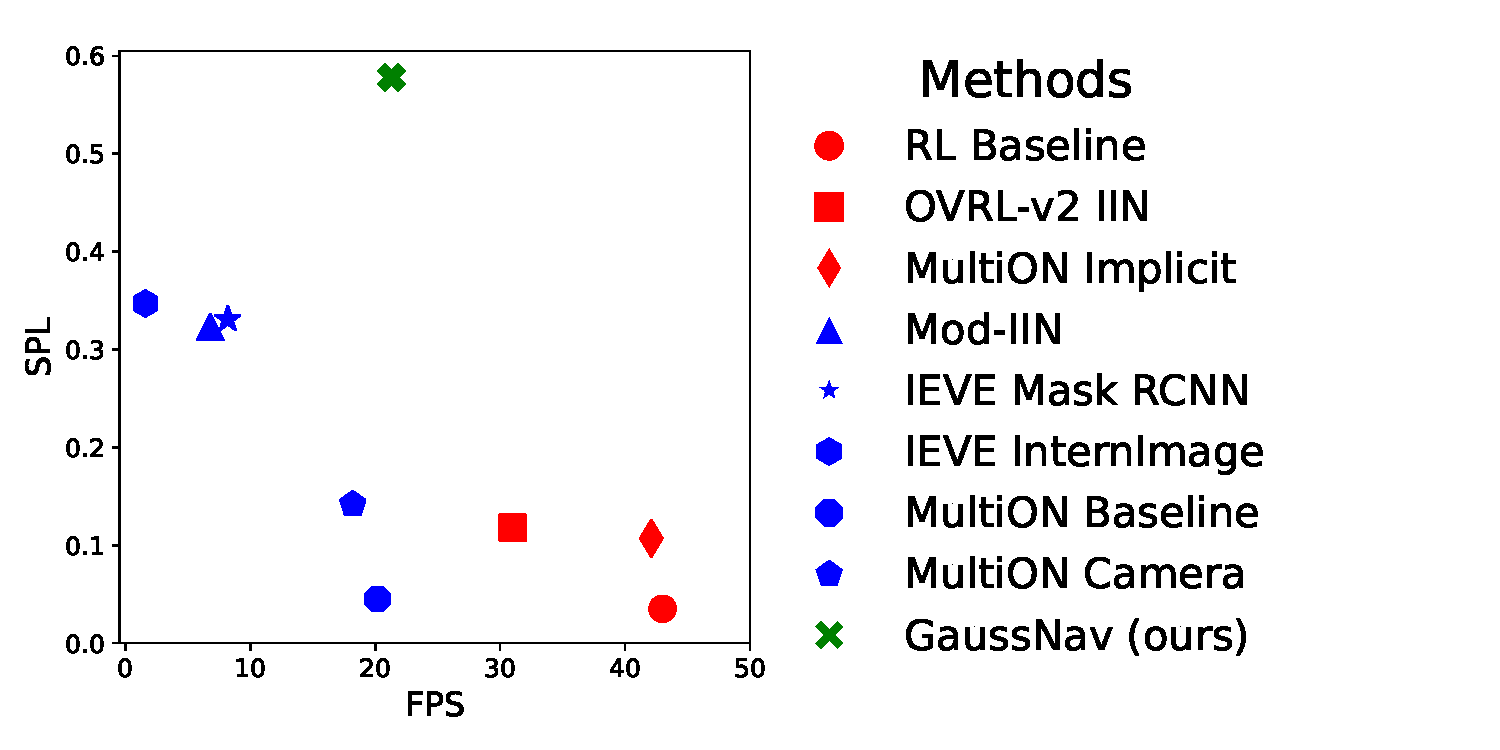
\includegraphics[width=0.45\textwidth]{pics/framerate.pdf}
\caption{SPL and FPS Analysis. {\color{red}Red markers} represent end-to-end methods, while {\color{blue}blue markers} indicate modular approaches. Our {\color{MyGreen}GaussNav} belongs to the modular approach, achieving the highest frame rate among modular methods while attaining the highest SPL across all approaches in IIN task.}
\vspace{-10pt}
\label{fig:framerate}
\end{figure}


\begin{figure*}
  \centering
  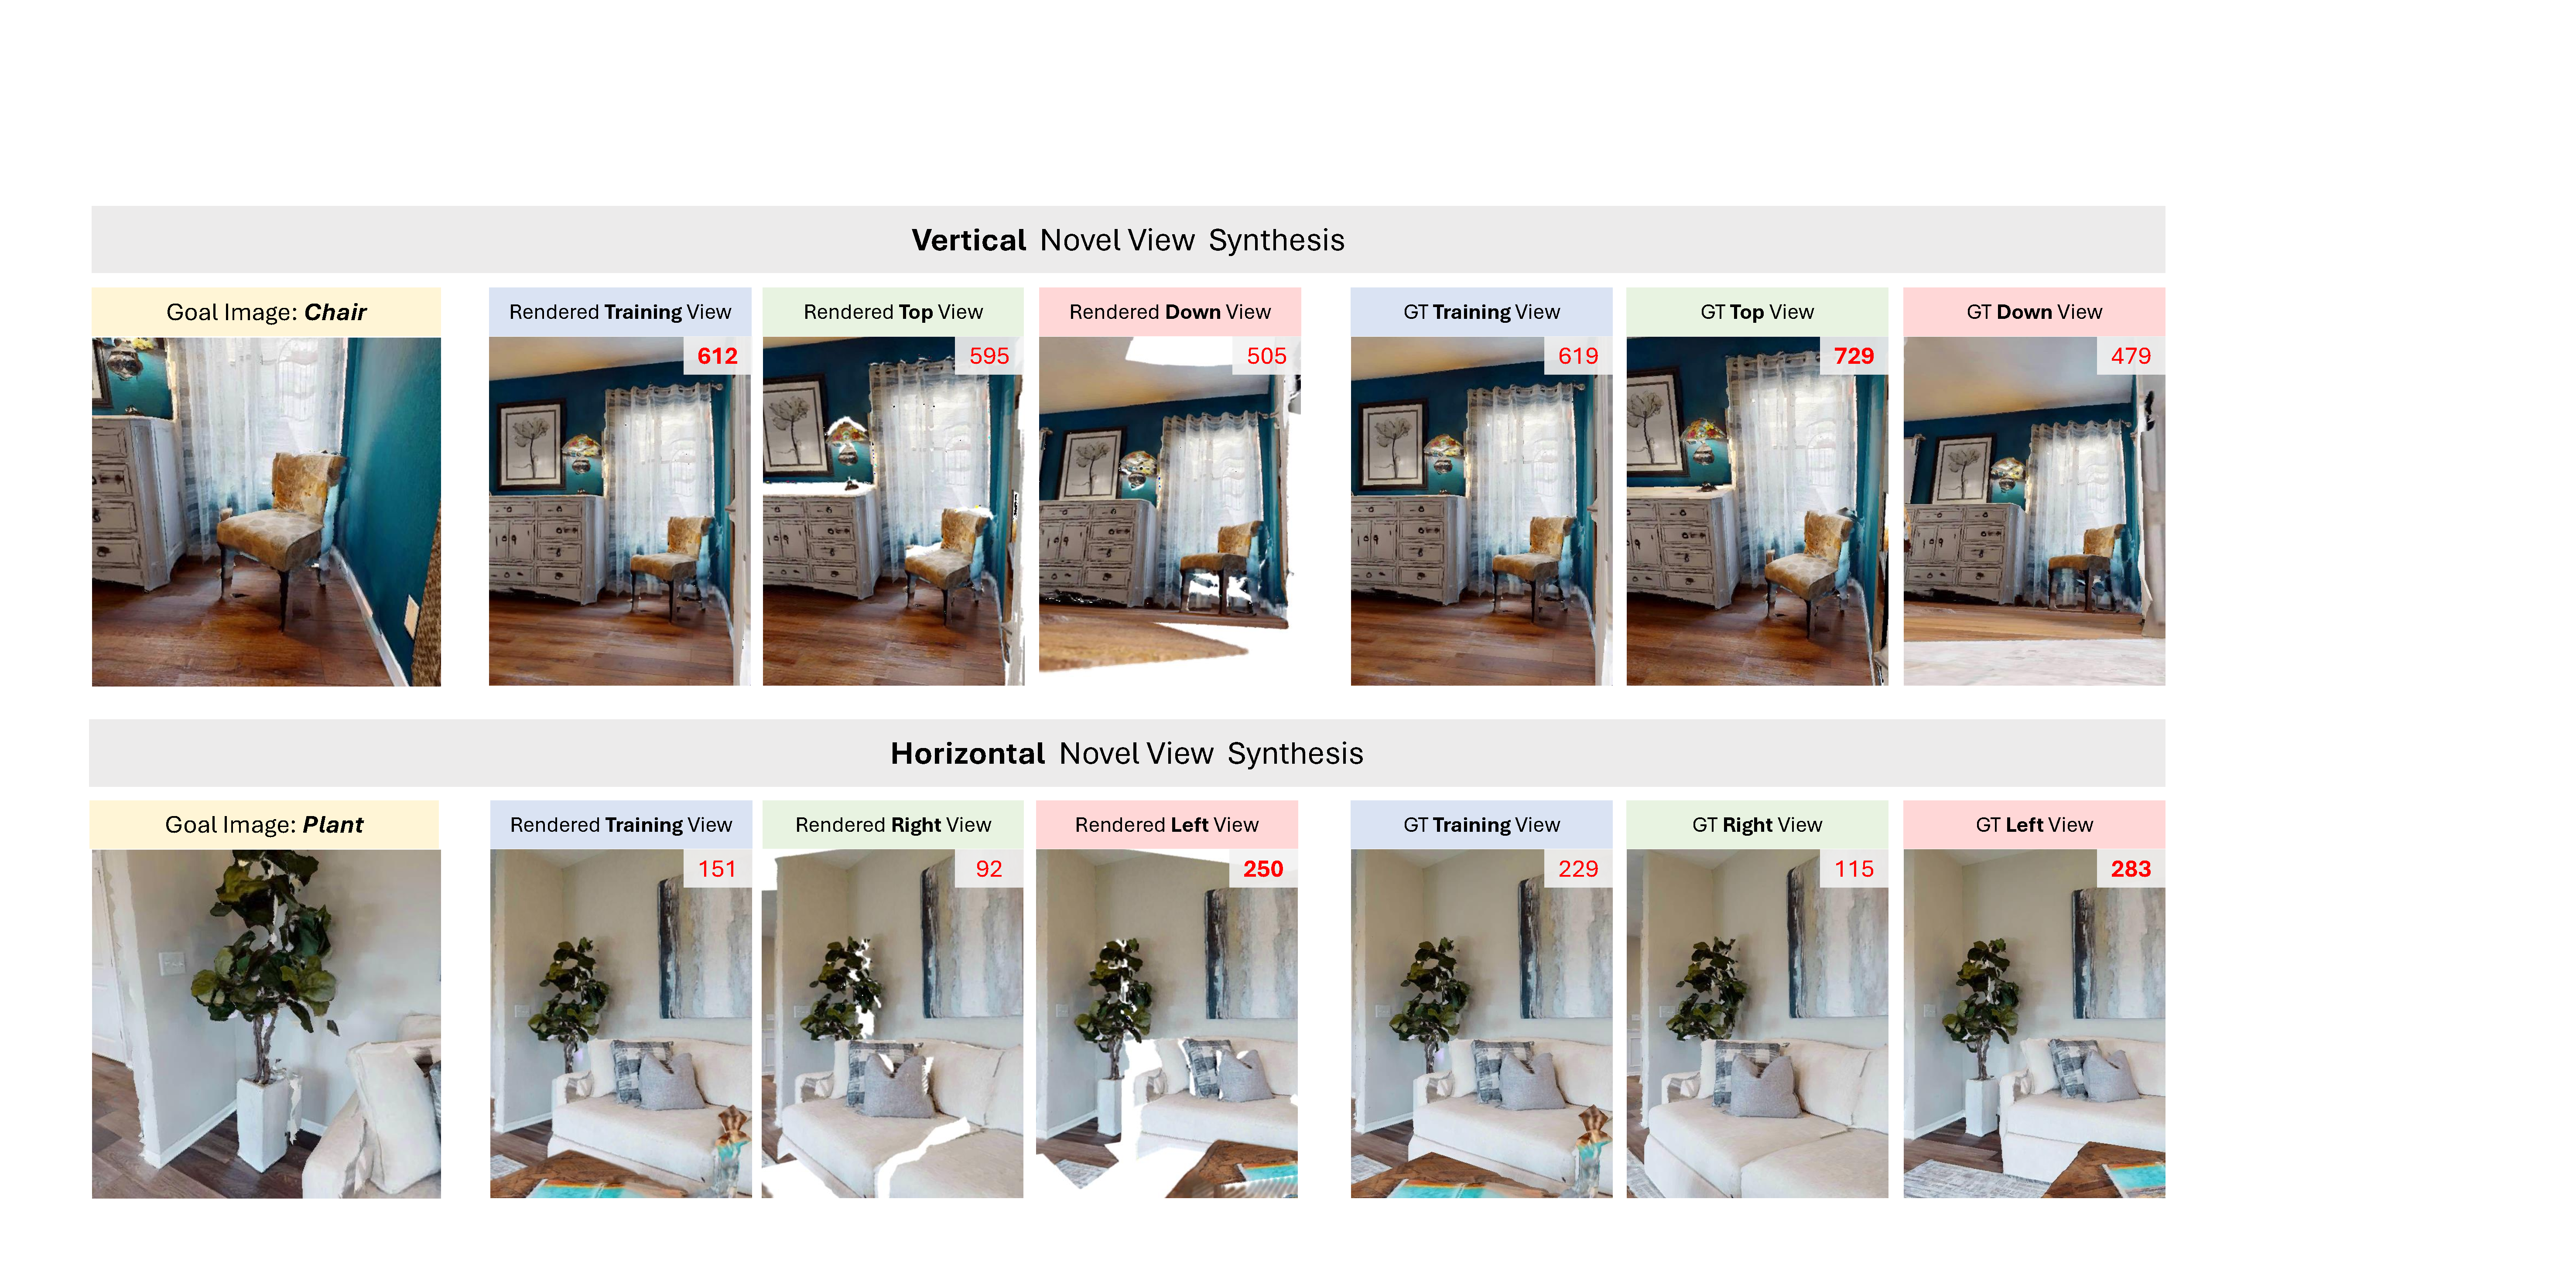
\includegraphics[width=0.95\linewidth]{pics/NVS.pdf}
  \vspace{-10pt}
  \caption{Visualization of novel view  synthesis results. The visualization results include horizontal and vertical novel view  synthesis results with $\theta = \pm15^\circ$. The upper right corner of each image shows the number of matched keypoints with the goal image.
  }
  \vspace{-6pt}
  \label{fig:NVS}
\end{figure*}

\begin{table}[tb]
  \centering
  % Increase the padding of the columns
  % \setlength{\tabcolsep}{16pt}
  % Optionally, use a smaller font for the table
  \small
  % \vspace{-18pt}
  \vspace{6pt}
  \begin{tabular}{@{}c c c c c c@{}}
    \toprule
    Chair & Sofa & TV & Plant & Toilet & Bed \\
    \midrule
    11 & 2 & 1 & 3 & 1 & 0 \\
    \bottomrule
  \end{tabular}
  % \vspace{-10pt}
  \vspace{5pt}
  \caption{Number of object instances across different categories in the first floor of scene \texttt{CrMo8WxCyVb}.} 
  \vspace{-24pt}
  \label{tab:time}
\end{table}

\begin{table*}[tb]
    \renewcommand{\arraystretch}{1.2} % Increase the row height
    \centering
    \begin{tabular}{c cc cc cc cc cc}
        \hline
        \multirow{2}{*}{Metric} & original & GT original & \multicolumn{2}{c}{horizontal} & \multicolumn{2}{c}{vertical} & \multicolumn{2}{c}{GT horizontal} & \multicolumn{2}{c}{GT vertical} \\
        \cline{2-11}
        & $n_v=1$ & $n_v=1$ & $n_v=3$ & $n_v=5$ & $n_v=3$ & $n_v=5$ & $n_v=3$ & $n_v=5$ & $n_v=3$ & $n_v=5$ \\
        \hline
        Success $\uparrow$ & 0.811 & 0.815 & 0.824 & 0.827 & 0.832 & 0.831 & 0.835 & 0.846 & 0.839 & 0.845 \\
        Time (s) $\downarrow$ & 11.5 & 11.7 & 32.1 & 53.9 & 33.1 & 54.2 & 32.7 & 54.1 & 33.4 & 55.1 \\
        \hline
    \end{tabular}
    \vspace{5pt}
    \caption{Results of the number of rendered images $n$, different directions (vertical or horizontal) and whether to use ground truth rendering's impact on the matching success.}
    \vspace{-16pt}
    \label{tab:NVS}
\end{table*}

% \begin{table*}[tb]
%     \centering
%     \begin{tabularx}{\textwidth}{>{\raggedright\arraybackslash}p{2cm}*{10}{>{\centering\arraybackslash}X}}
%         \hline
%         \multirow{2}{*}{Metric} & o. & GT o. & \multicolumn{2}{c}{hor.} & \multicolumn{2}{c}{ver.} & \multicolumn{2}{c}{GT hor.} & \multicolumn{2}{c}{GT ver.} \\
%         \cline{2-11}
%         & $n_v=1$ & $n_v=1$ & $n_v=3$ & $n_v=5$ & $n_v=3$ & $n_v=5$ & $n_v=3$ & $n_v=5$ & $n_v=3$ & $n_v=5$ \\
%         \hline
%         Success $\uparrow$ & 0.811 & 0.815 & 0.824 & 0.827 & 0.832 & 0.831 & 0.835 & 0.846 & 0.839 & 0.845 \\
%         Time (s) $\downarrow$ & 11.5 & 11.7 & 32.1 & 53.9 & 33.1 & 54.2 & 32.7 & 54.1 & 33.4 & 55.1 \\
%         \hline
%     \end{tabularx}
%     \caption{Results of the number of rendered images $n$, different directions (ver. or hor.) and the impact of using ground truth rendering on matching success. The o.\ means the original training view, \textit{hor.} indicates horizontal NVS, and \textit{ver.} represents vertical NVS. $n$ is the number of rendered images.}
%     \label{tab:NVS}
% \end{table*}

% \begin{table*}[tb]
%     \renewcommand{\arraystretch}{1.2} % Increase the row height
%     \centering
%     % \large % Increase the font size within the table
%     \begin{tabularx}{\textwidth}{>{\raggedright\arraybackslash}p{2.5cm}*{10}{>{\centering\arraybackslash}X}}
%         \hline
%         \multirow{2}{*}{Metric} & o. & GT o. & \multicolumn{2}{c}{hor.} & \multicolumn{2}{c}{ver.} & \multicolumn{2}{c}{GT hor.} & \multicolumn{2}{c}{GT ver.} \\
%         \cline{2-11}
%         & $n_v=1$ & $n_v=1$ & $n_v=3$ & $n_v=5$ & $n_v=3$ & $n_v=5$ & $n_v=3$ & $n_v=5$ & $n_v=3$ & $n_v=5$ \\
%         \hline
%         Success $\uparrow$ & 0.811 & 0.815 & 0.824 & 0.827 & 0.832 & 0.831 & 0.835 & 0.846 & 0.839 & 0.845 \\
%         Time (s) $\downarrow$ & 11.5 & 11.7 & 32.1 & 53.9 & 33.1 & 54.2 & 32.7 & 54.1 & 33.4 & 55.1 \\
%         \hline
%     \end{tabularx}
%     \caption{Results of the number of rendered images $n$, different directions (ver.\ or hor.), and the impact of using ground truth rendering on matching success. The o.\ means the original training view, \textit{hor.} indicates horizontal NVS, and \textit{ver.} represents vertical NVS. $n$ is the number of rendered images.}
%     \label{tab:NVS}
% \end{table*}



\subsection{Ablation Study}




To understand the modules of our GaussNav, we consider the following ablations:

\textbf{GaussNav w.o. Classifier.} In \Cref{fig:main}, we replace the Classifier's output with a random generated target category. We observe that the Success drops to 0.375 and the SPL decreases to 0.291 (row 2 in \Cref{tab:ablations}). To better evaluate the classifier, we design the following experiment. We define the training views from the full space of candidate objects as the complete set, and the training views filtered by the classifier as a subset. Given the goal image and the keypoint matcher, we compute, in each set respectively, the view with the largest number of matching keypoints. If this view contains the goal object, we consider it a success; otherwise, a failure. We also record the total time spent in the entire local feature matching process to assess the impact of the classifier on efficiency. Here, we do not use the navigation metrics such as Success and SPL because this allows us to eliminate the influence of irrelevant factors, such as path planning errors. Our experimental results are shown in \Cref{tab:abla_classifier}. As can be seen, the total success without the classifier is slightly higher than that with the classifier (an increase of 0.039), but the improvement is limited. However, the time taken is 2.5 times that with the classifier, making it significantly less efficient. Therefore, considering the trade-off between performance and efficiency, we choose to include the classifier as a component of GaussNav framework.


% This is because correct classification is a prerequisite for our method to filter potential candidates.

\textbf{GaussNav w.o. Match.} The Match module is designed to distinguish the target from candidates with the same class. Without the Match module, we randomly select from these candidates. The Success and SPL falls to 0.444 and 0.353 (row 3 in \Cref{tab:ablations}). This can be attributed to the random selection of candidate instances without Match module.

\textbf{GaussNav w. SIFT or GlueStick \cite{pautrat_suarez_2023_gluestick}.} To evaluate the impact of different extractors and matching algorithms on our GaussNav, we replace the combination of DISK \cite{tyszkiewicz2020disk} + LightGlue \cite{lindenberger2023lightglue}. We employ both SIFT + FLANN and GlueStick \cite{pautrat_suarez_2023_gluestick} as alternatives. The first replacement represents a greater decrease, (row 4 in \Cref{tab:ablations}) and the second only displays a slight decrease (row 5 in \Cref{tab:ablations}). These results demonstrate the varying performance of different local feature matching algorithms on the HM3D dataset.

\textbf{NVS Analysis.} We conduct experiments to evaluate the impact of the number of rendered images $n_v$ and the upper bound of NVS. Specifically, we perform ablation studies on NVS with $n_v=3$ and $n_v=5$ in both horizontal and vertical directions, and also evaluate the upper bound achievable using GT rendered results. To avoid the influence of other factors in navigation, we consider it a success only if the image retrieved through keypoint matching contains the target object; otherwise, it is considered a failure. The specific evaluation metrics are detailed in \textbf{GaussNav w.o. Classifier.}. The experimental results are presented in \Cref{tab:NVS}. Overall, utilizing NVS is beneficial for successfully recognizing objects. However, a large $n_v$ does not necessarily yield positive effects (see \Cref{tab:NVS}, vertical $n_v=5$ \textit{vs.} vertical $n_v=3$). This is because our Semantic Gaussian map may have only a few observational viewpoints for a particular object, unlike the dozens available in traditional 3DGS. Therefore, when rendering from novel viewpoints, artifacts such as holes may occur, reducing the number of features, as visualized in \Cref{fig:NVS}. Nevertheless, for GT NVS, the improvement is significant.

\begin{table}[tb]
    \centering
    \vspace{5pt}
    \begin{tabular}{l c c c c c}
        \toprule
         Method & Ver. NVS & Hor. NVS & GT & Success~$\uparrow$ & SPL~$\uparrow$  \\
         \midrule
         IEVE~\cite{lei2024instanceaware} & - & - & - & 0.702 & 0.252 \\
         GaussNav (ours) & $\checkmark$ & $\times$ & $\times$ & 0.713 & 0.259 \\
         GaussNav (ours) & $\times$ & $\checkmark$ & $\times$ & 0.715 & 0.261 \\
         GaussNav (ours) & $\checkmark$ & $\checkmark$ & $\times$ & 0.723 & 0.265 \\
         GaussNav (ours) & $\checkmark$ & $\checkmark$ & $\checkmark$ & 0.747 & 0.289 \\
         \bottomrule
    \end{tabular}
    \vspace{-1pt}
    \caption{Performance Comparison of IEVE~\cite{lei2024instanceaware} and GaussNav. We compare GaussNav with the state-of-the-art method IEVE using different map representations. (Abbreviations: Ver. = Vertical, Hor. = Horizontal)}
    \vspace{-30pt}
    \label{tab:pre-exploration}
\end{table}

To further study the impact of NVS without pre-exploration, we adopt the same framework as IEVE~\cite{lei2024instanceaware}, with the only difference being the map representation. IEVE uses 2D BEV map while GaussNav implements Semantic Gaussian map. Additionally, GaussNav performs NVS whenever a similar object appears in each observation. The results are presented in \Cref{tab:pre-exploration}. Our Semantic Gaussian map enhances the existing observations without relying on pre-exploration. While the improvement may not be as prominent as the ability of instance-level object localization, the result of last row in \Cref{tab:pre-exploration} indicates promising direction for future work.

\subsection{Efficiency Analysis}

\begin{figure*}
  \centering
  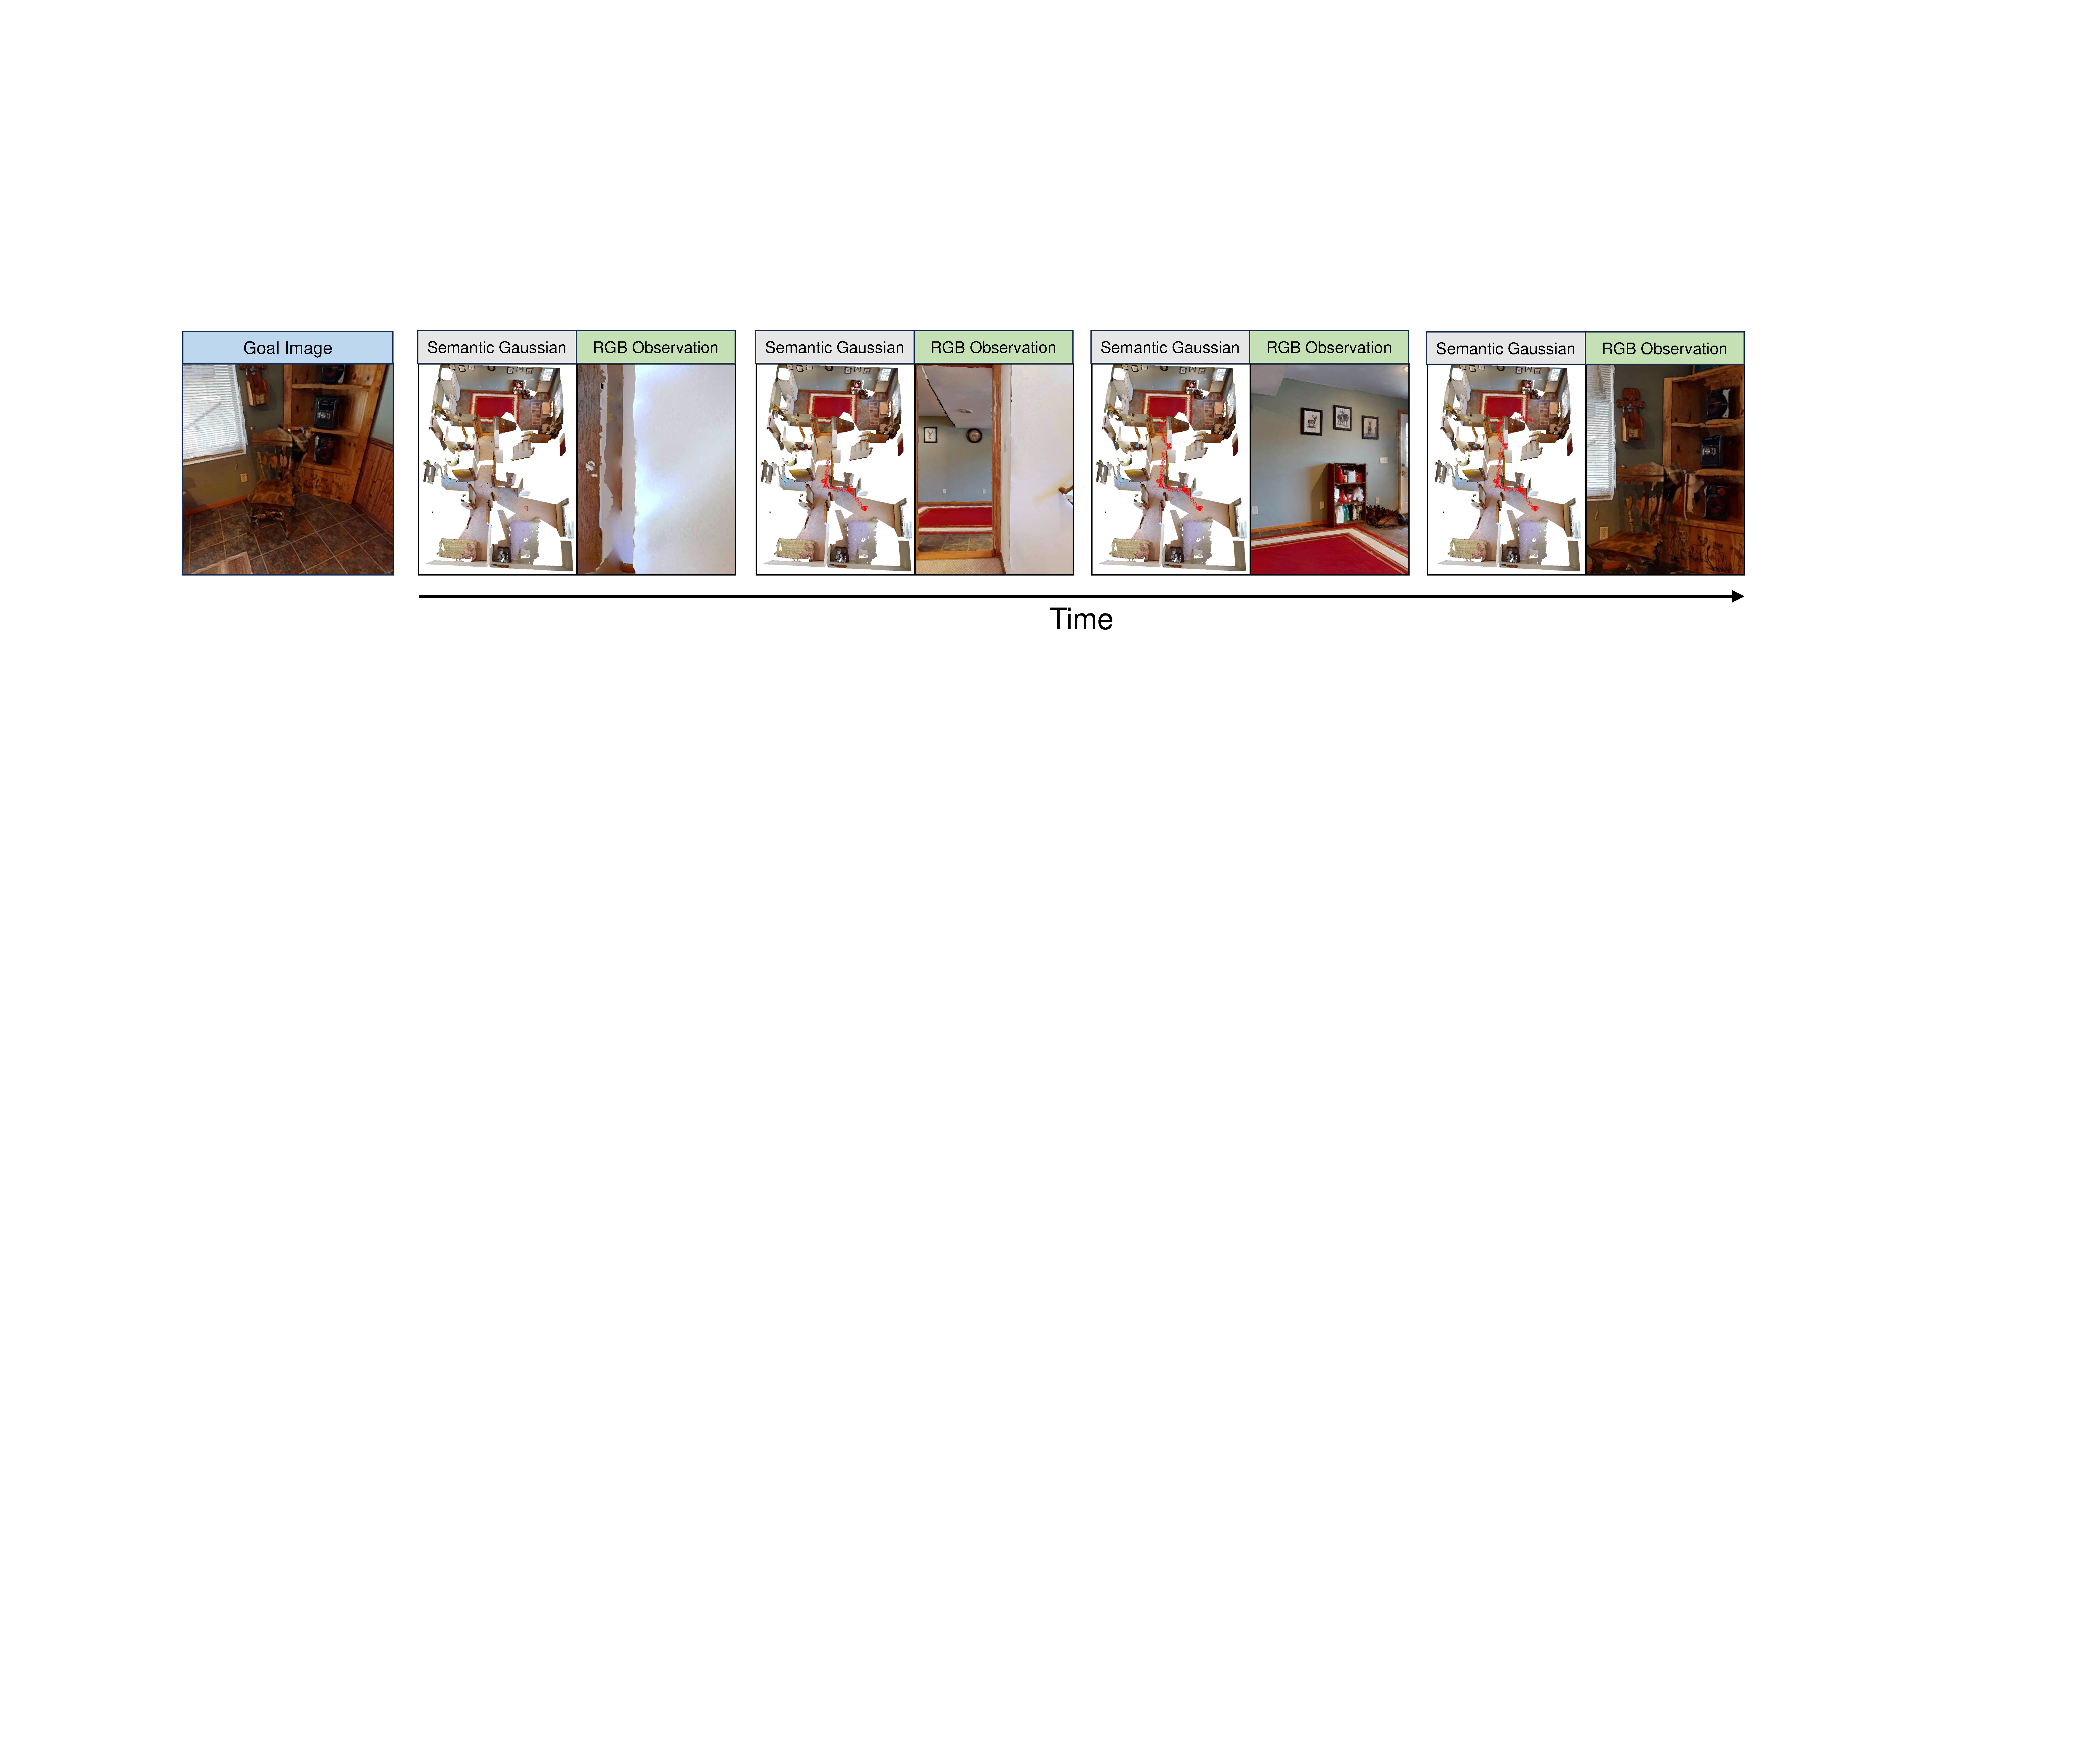
\includegraphics[width=0.95\linewidth]{pics/qualitive_result.pdf}
  \vspace{-10pt}
  \caption{Qualitative example of our GaussNav agent performing IIN task in the Habitat simulator. When randomly initialized in the environment, the agent is given a goal image depicted a target object. Gaussian Navigation directly grounds the target object in the Semantic Gaussian and guide the agent towards it.
  }
  \vspace{-10pt}
  \label{fig:qualitive_result}
\end{figure*}

\begin{figure*}
  \centering
  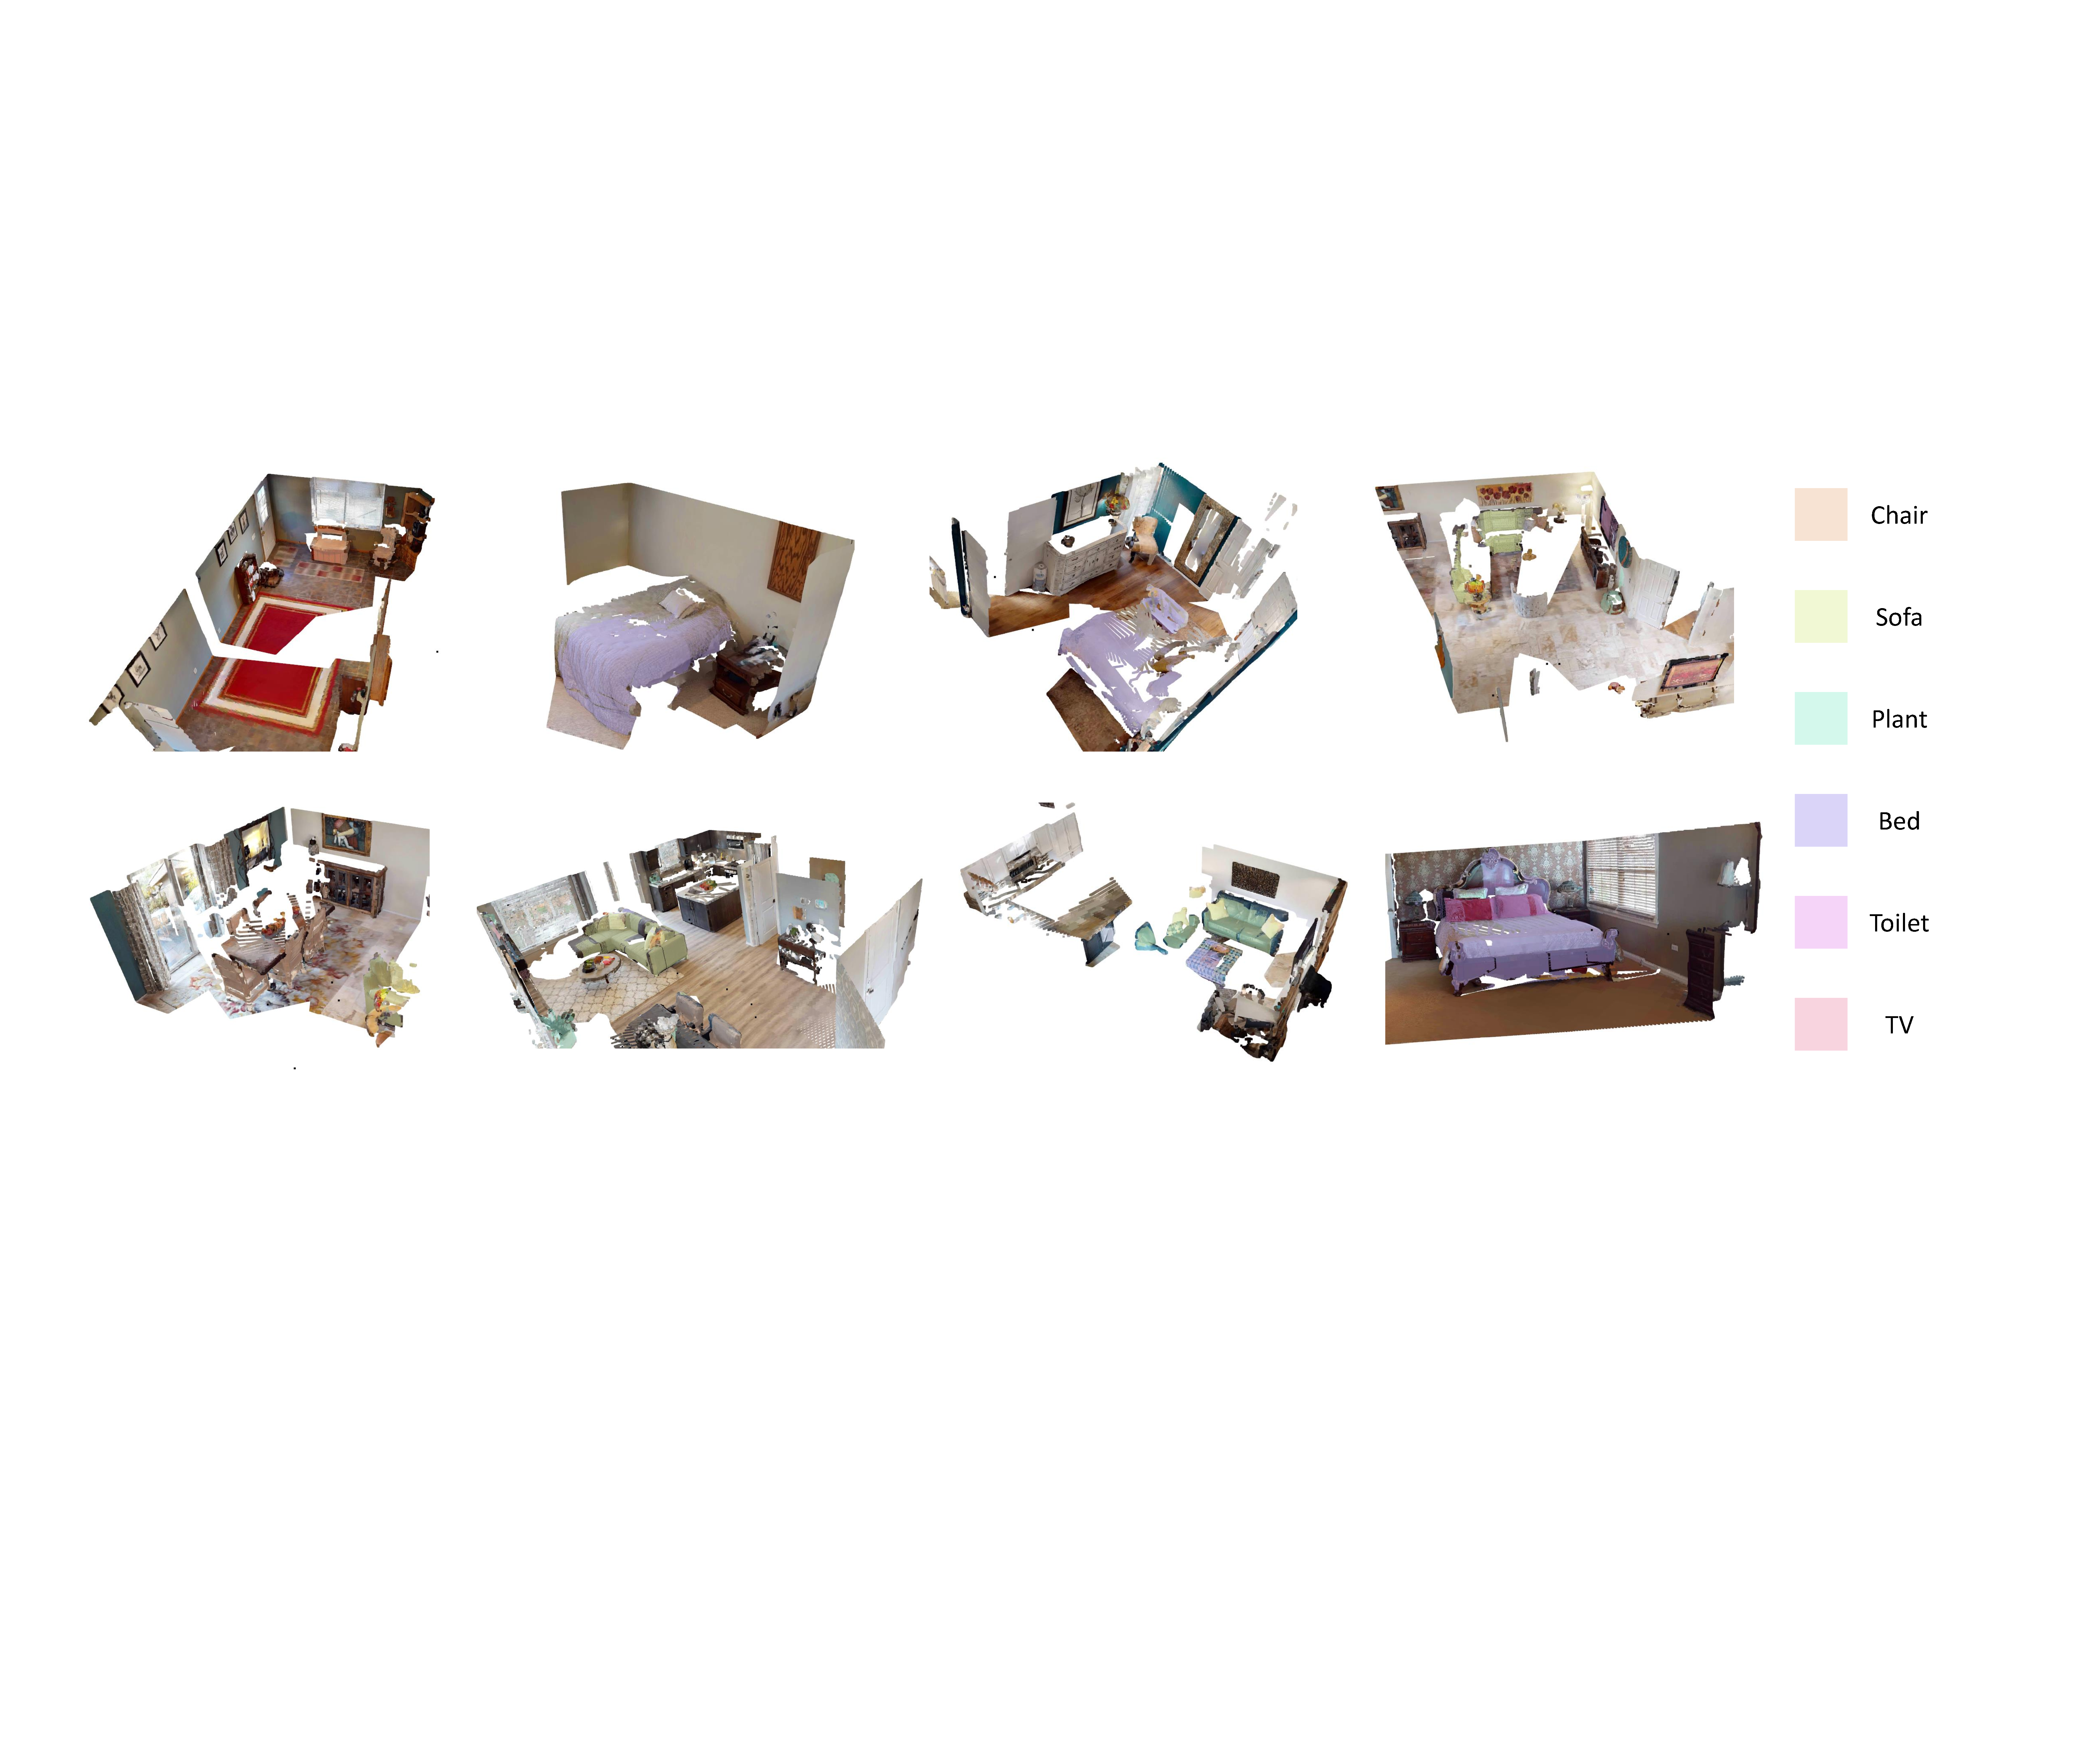
\includegraphics[width=0.95\linewidth]{pics/supp_gauss.pdf}
  \caption{Semantic Gaussian visualization results.
  }
  \vspace{-6pt}
  \label{fig:vis_gauss}
\end{figure*}


We analyze the temporal efficiency of our approach from two perspectives: preprocessing and agent-environment interaction. In the context of our method, ``preprocessing'' refers to the process of matching and grounding target objects given the Semantic Gaussian. The latter perspective compares the runtime frame rate of our method with various other approaches.


Efficiently locating the target object within the map is crucial for our method, which leverages renderings to match and ground the goal object. To reduce the computational cost of comparing all possible observations at each navigable viewpoint, we introduce Semantic Gaussians. This technique groups object instances under their corresponding semantic labels. This optimization significantly reduces the search space by limiting comparisons to several descriptive renderings of each instance. For example, in the scene \texttt{CrMo8WxCyVb}, the navigable area is quantified to be $54.03 m^2$. This space can be discretized into approximately 54 squares, each with an area of $1 m^2$. Positioned within each square, the agent can observe its surroundings from 12 distinct viewing angles, covering a full $360 \deg$ with each angle spanning $30 \deg$. Thus, the original search space for this single floor would consist of $12 \times 54 = 648$ potential observations. By applying our grouping strategy based on semantic labeling, the search space is considerably narrowed. We count the number of different categories of object instances within the \texttt{CrMo8WxCyVb} scene, as demonstrated in \Cref{tab:time}. To locate a ``chair'' — assuming we render each object instance from three unique viewpoints — the resulting search space is reduced to merely $3 \times 11 = 33$ observations. We render three observations of a single instance to ensure rendering quality, which is achievable only when the new viewpoint largely overlaps with the training views. This optimization yields a significant improvement in time efficiency.

\begin{figure*}
  \centering
  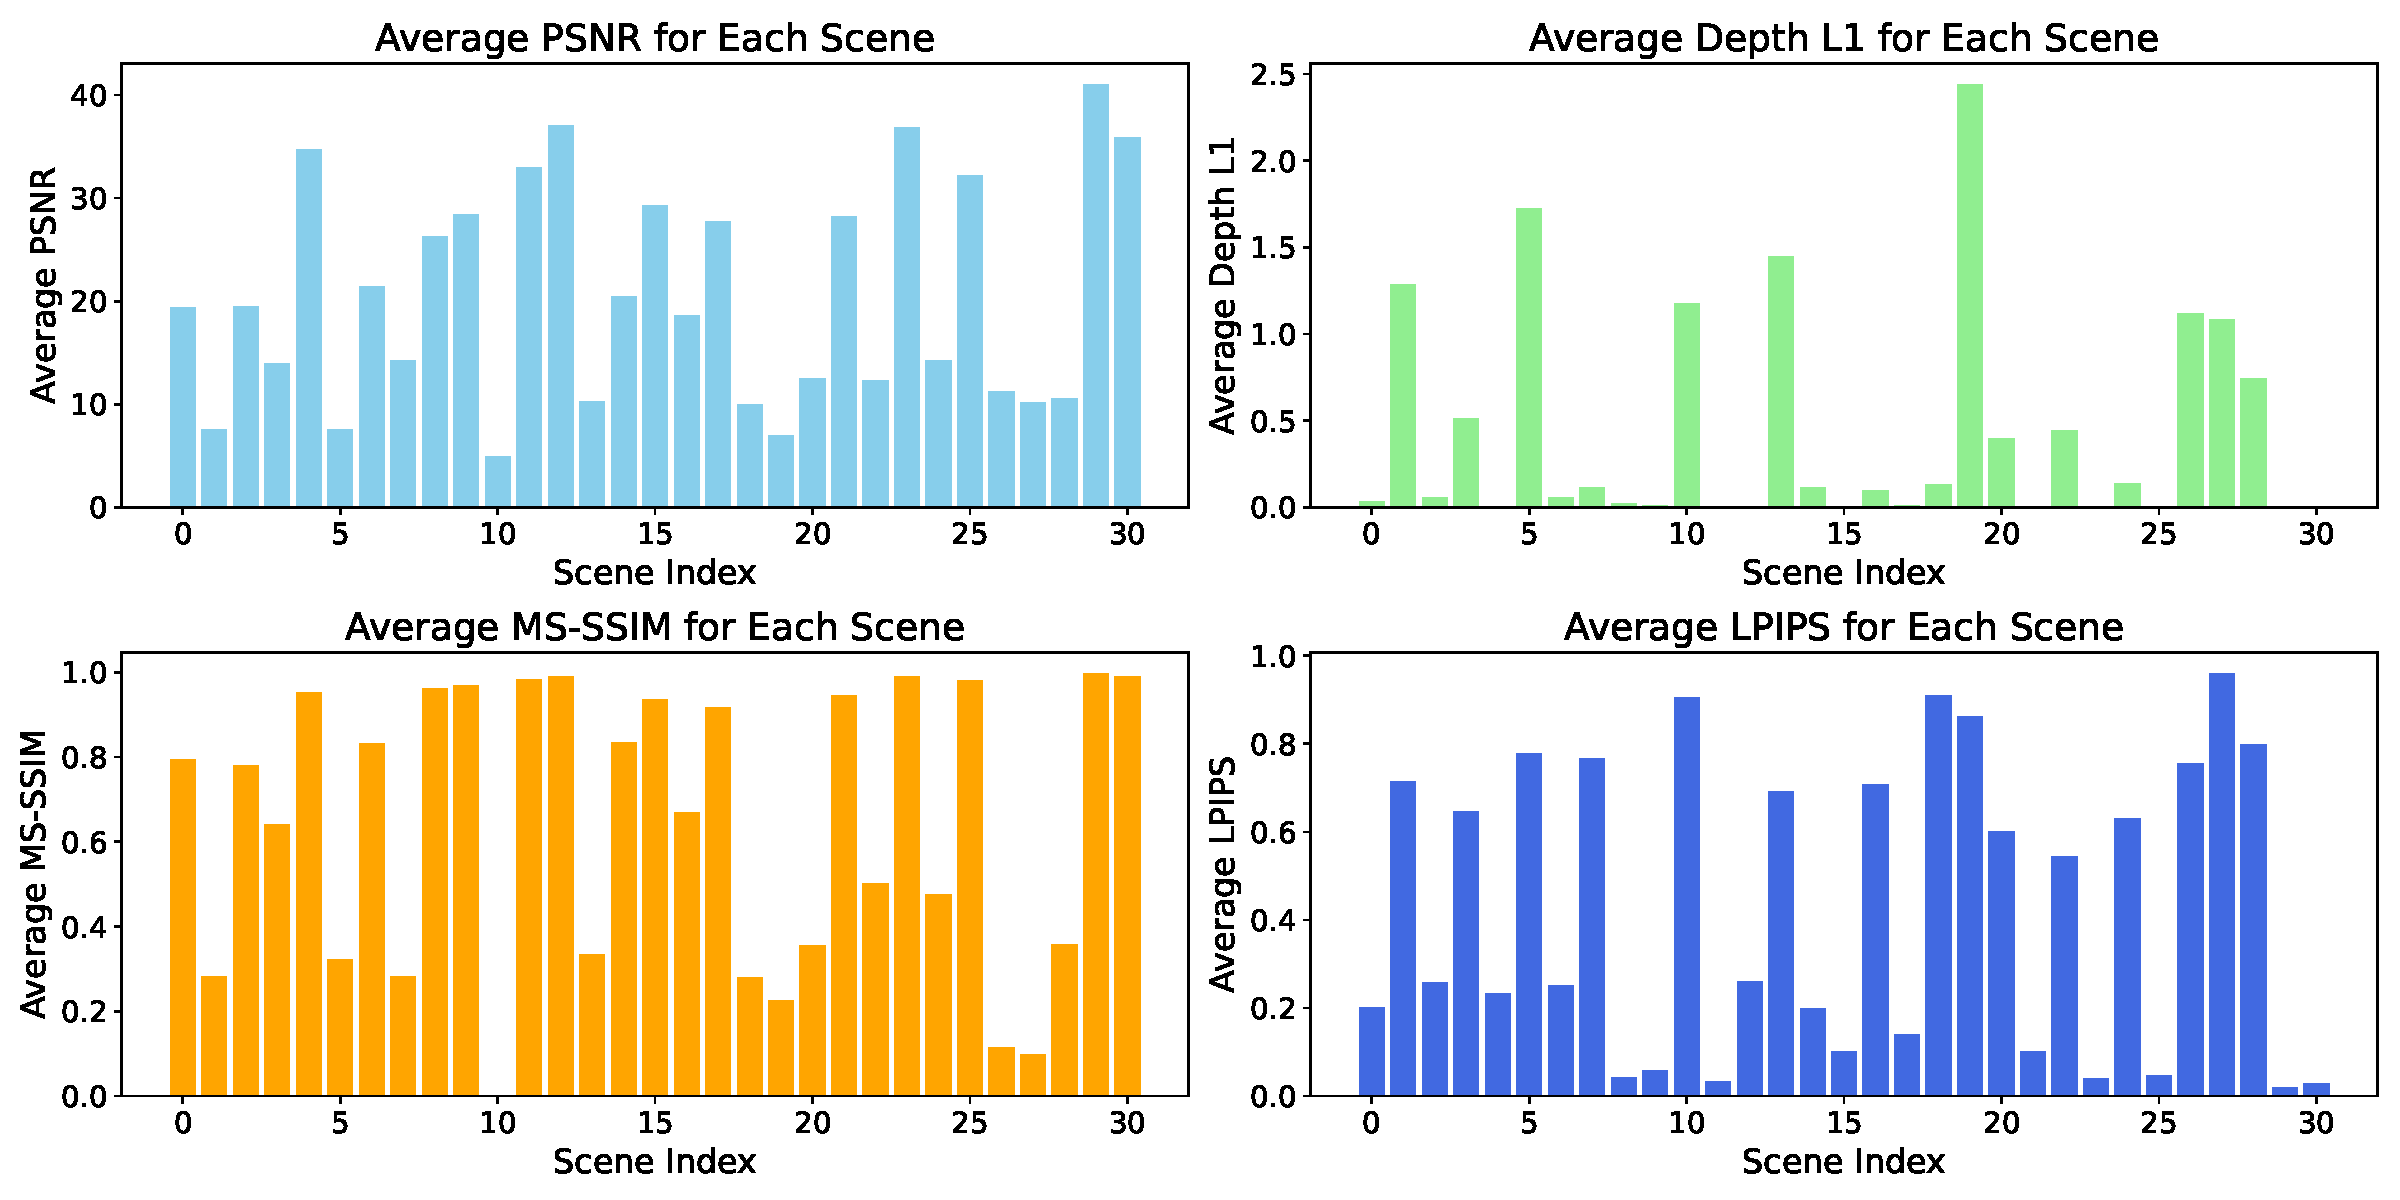
\includegraphics[width=0.99\linewidth]{pics/gauss.pdf}
  \caption{Rendering quality of our Semantic Gaussian Construction results on the HM3D validation dataset. The x-axis indicates different scene indices with the corresponding floor height.
  }
  \vspace{-4pt}
  \label{fig:gauss_results}
\end{figure*}

\begin{figure*}
  \centering
  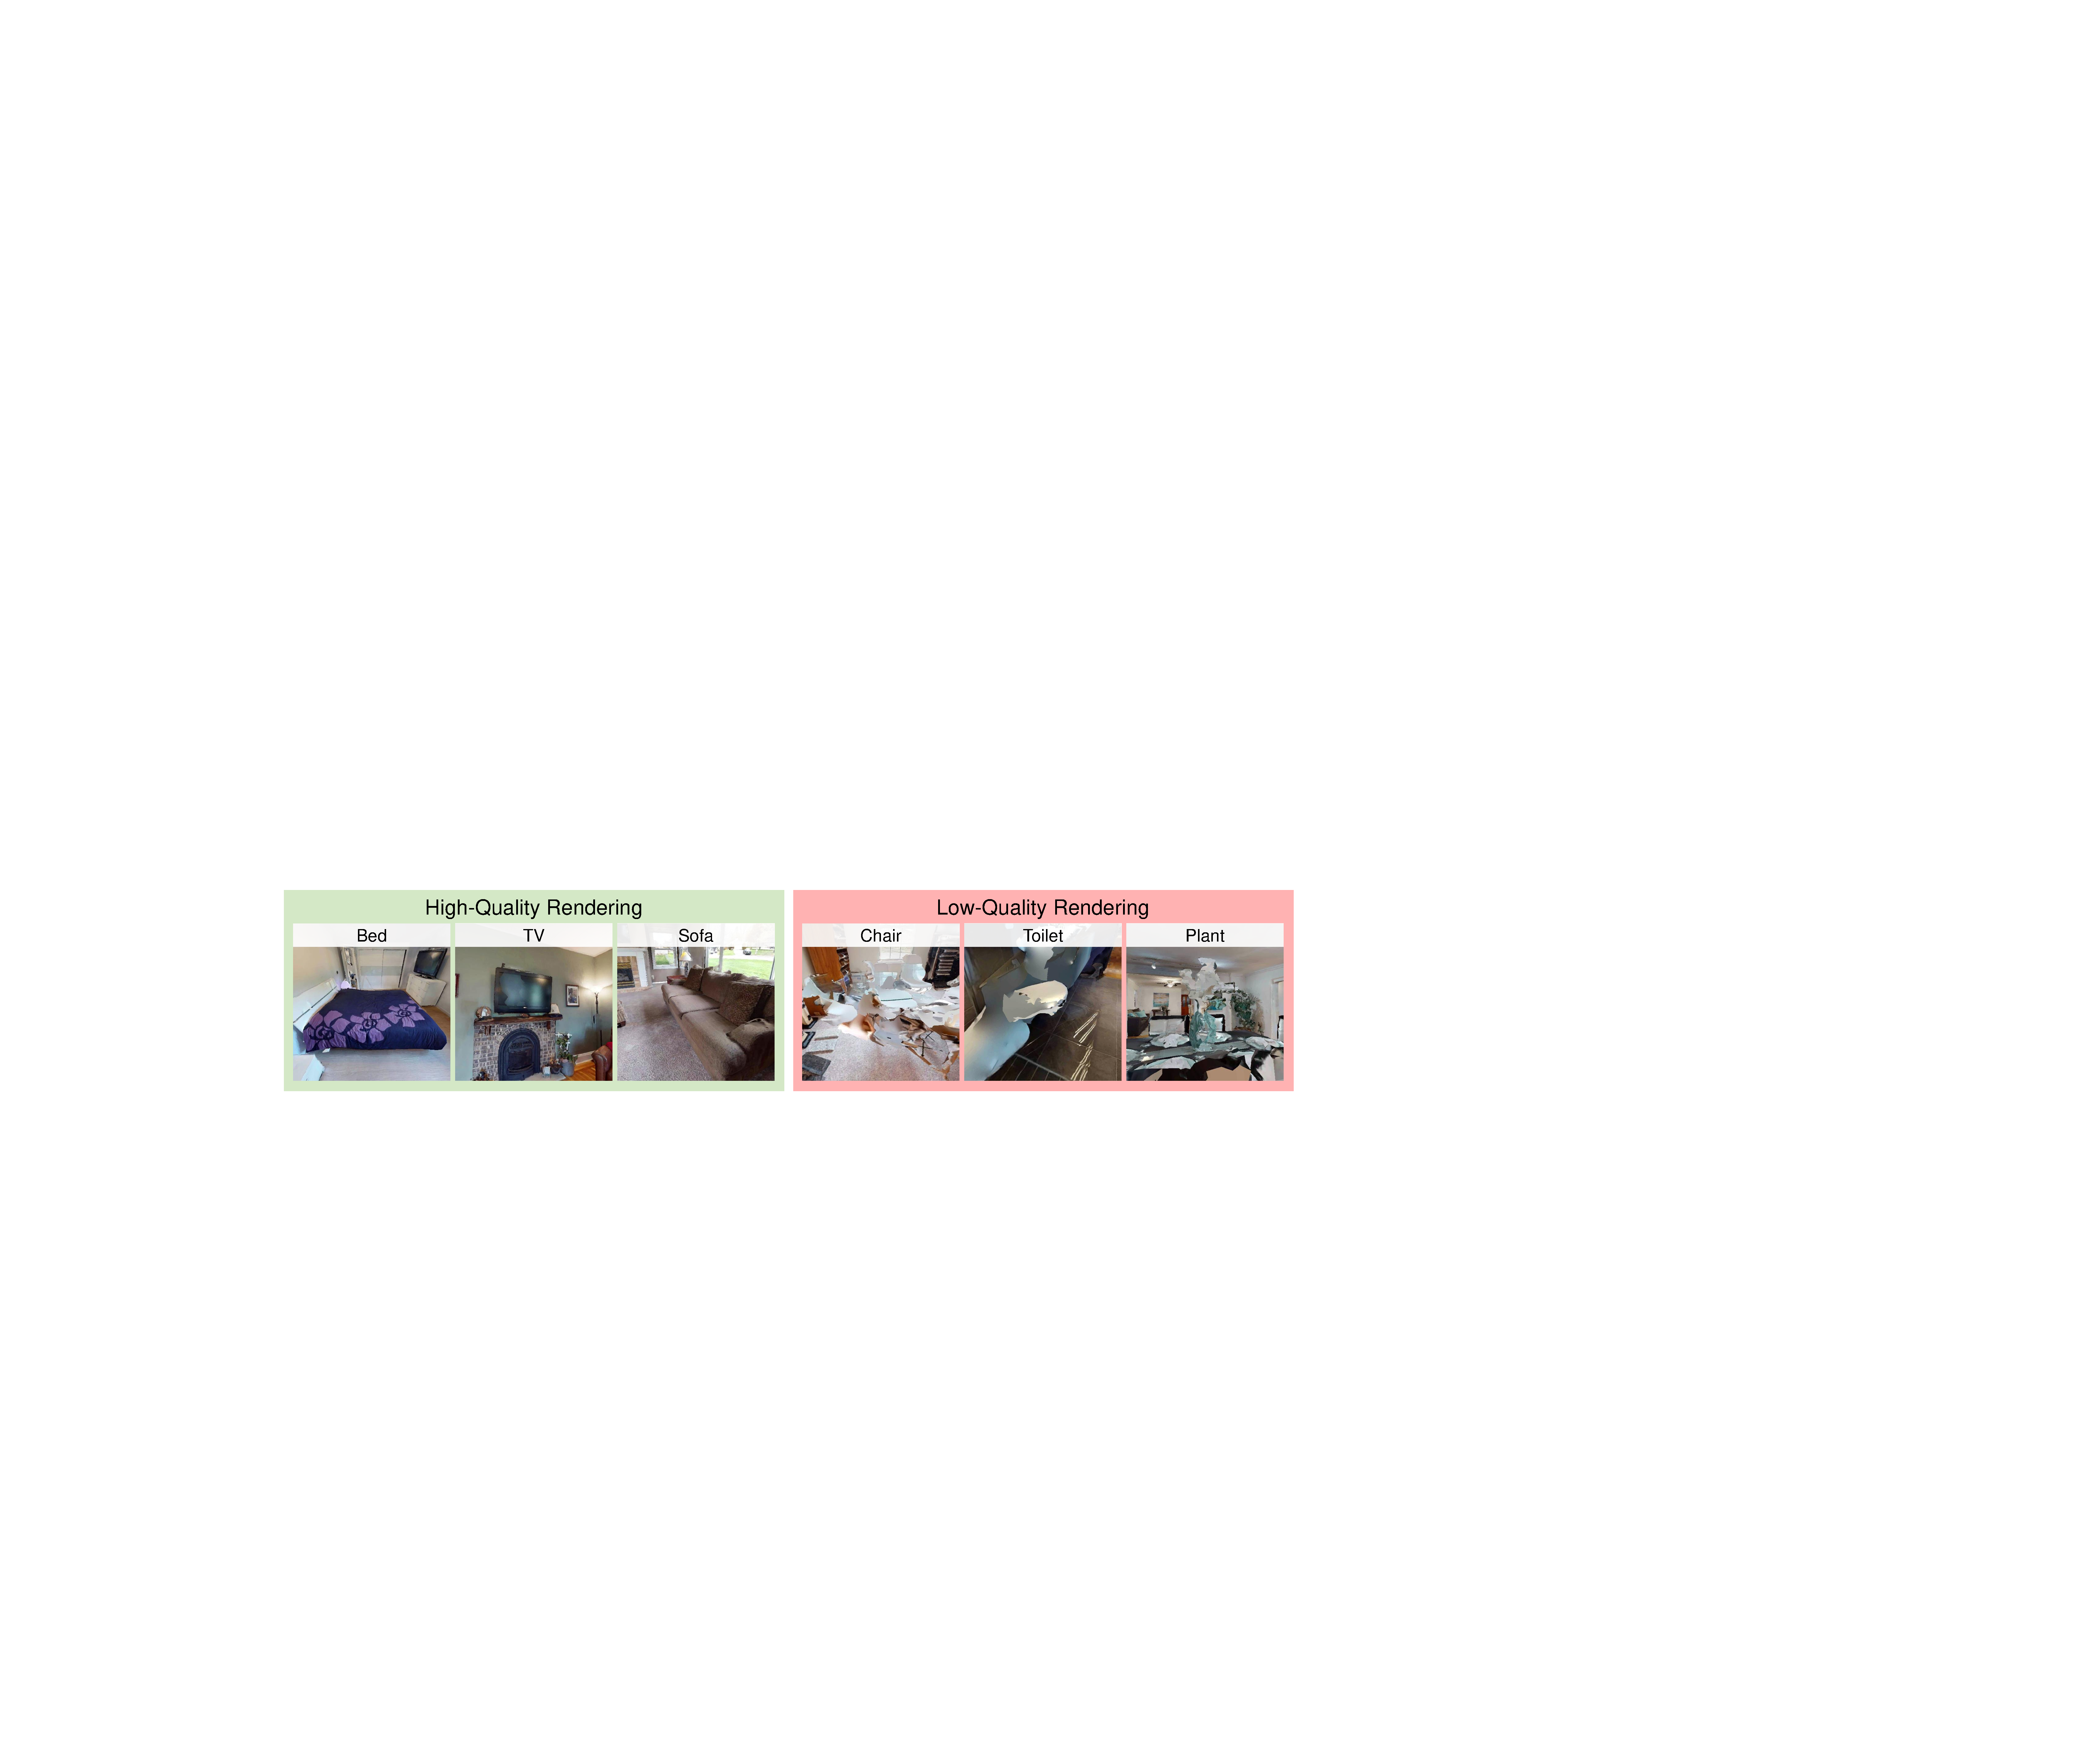
\includegraphics[width=0.99\linewidth]{pics/bad_render.pdf}
  \caption{Observations rendered from HM3D \cite{yadav2023habitat} scene dataset using the Habitat \cite{szot2022habitat} simulator.
  }
  \vspace{-16pt}
  \label{fig:bad_render}
\end{figure*}

We also compare the runtime frame rates of different methods in a single Habitat environment using an NVIDIA GeForce RTX 3090 GPU and 10 CPU cores. As shown in \Cref{fig:framerate}, our method maintains a high efficiency of over 20 FPS while achieving the highest SPL among the compared approaches. To achieve higher runtime speed, our GaussNav projects the Semantic Gaussian to obtain a 2D grid map. By utilizing the predicted target location from the ``preprocessing'', we then employ Fast Marching Method (FMM) for path planning. The reason why our method outperforms various Modular Methods in terms of speed is that we do not rely on additional modules such as semantic segmentation \cite{krantz2023navigating, lei2024instanceaware}, local feature matching \cite{krantz2023navigating, lei2024instanceaware}, or switch module \cite{lei2024instanceaware} during the navigation. This simplification enables GaussNav to operate more efficiently. We also provide a qualitative example of our GaussNav navigating to the target object instance, as depicted in \Cref{fig:qualitive_result}.



\subsection{Error Analysis}

The performance of the proposed model is still far from perfect. We would like to understand the error modes for future improvements. Our analysis identifies two sources of error: the first being the model's inability to consistently match the target from instance renderings, and the second, inaccuracies in goal localization. To quantify the impact of these error sources, we conduct an evaluation of our model using a ground truth Match module and an accurate goal localization. The first one means agent can correctly recognize the target from candidate observations, and the second suggests agent is directly provided with the ground truth goal position. The variant equipped with a ground truth Match module (\textbf{GaussNav w. GT Match} in \Cref{tab:ablations}) shows that Success can be enhanced by approximately 0.127 (rows 5 and 6 in \Cref{tab:ablations}). Furthermore, when the model is augmented with both ground truth Match and Goal Localization, denoted as \textbf{GaussNav w. GT Goal Localization}, we observe an increase in Success from 0.850 to 0.946, as indicated in rows 6 and 7 in \Cref{tab:ablations}. Improvements in the first error source may be achievable through the development of a more robust re-identification algorithm. As for the second source, a more precise Grounding strategy could yield better results. These insights not only highlight the model's current shortcomings but also chart a course for subsequent refinement efforts.

\vspace{-3pt}


\subsection{Gaussian Construction Results}



As illustrated in \Cref{fig:vis_gauss}, we provide visualization results of our Semantic Gaussian. These examples demonstrate the effectiveness of our Semantic Gaussian representation across a diverse range of scenarios. By presenting a more extensive collection of results, we aim to showcase the robustness and applicability of our approach in handling various scene complexities and object compositions.

In \Cref{fig:gauss_results}, we present an quantitative evaluation of the rendering quality produced by our Semantic Gaussian Construction method on the HM3D validation dataset \cite{yadav2023habitat}. To align with the constraints of IIN task \cite{krantz2022instancespecific}, we divide each scene within HM3D into separate floors and restrict the agent's movement to within a single floor, as the IIN task \cite{krantz2022instancespecific} inherently ensures that both the agent's starting location and the target's position are on the same floor.

To quantitatively analyze the results in \Cref{fig:gauss_results}, we observe that the rendering results exhibit a bifurcated trend. For instance, in scenes with indices 29 and 30, the rendered images achieve a high PSNR of up to 40 and a near-zero depth rendering error. However, the rendering performance for scene 10 is suboptimal. We hypothesize that this polarized rendering quality across different scenes can be attributed to the discrepancy between the simulation and reality. This is evident in \Cref{fig:bad_render}, where some renderings from the HM3D dataset using Habitat simulator exhibit low fidelity, particularly in highly textured environments. High-quality reconstruction in such intricate settings is difficult, and utilizing suboptimal renderings as a basis for 3D environment reconstruction can further degrade the quality of the final output. In light of this, for scenes that are poorly reconstructed, we maintain consistency by using the original training views, rather than attempting to render novel views which would likely result in a diminished quality.







